\documentclass[12pt,notitlepage]{article}
\usepackage[bitstream-charter]{mathdesign}
\usepackage{inconsolata}
\usepackage[T1]{fontenc}
\usepackage{microtype}
\usepackage{graphicx}
\usepackage[utf8x]{inputenc}
\usepackage[letterpaper]{geometry}
\usepackage{titlesec}

\titleformat{\section}{\normalfont\large}{\thesection}{1em}{}

\begin{document}
\begingroup
  \centering
  {\Large Proposal: Concreteness Fading and Visual Programming in
  Teaching Object-Oriented Programming\\[1em]}

  Andy Jiang, Michael Mauer, and David Li\par
\endgroup

\section{Problem Definition}

Much effort has gone towards methods to teach programming as an
overall concept, with systems like Alice, Scratch, and CodeSpells
demonstrating how visual programming can successfully introduce
students to this field. Our goal is to teach the more specific topic
of object-oriented programming to novice programmers using these same
techniques, focusing on how to abstract and represent ideas such as
inheritance, polymorphism, and interfaces in such a framework.
Additionally, to reinforce these concepts to an audience already
somewhat familiar with programming, we will introduce concreteness
fading to the system, transitioning students from visual programming
to directly writing code. This will facilitate the learning of these
specific higher-level concepts and abstractions within computer
science, which is important to effectively educate and train the next
generation of computer science and software development students.

\section{Approach}

Our approach is to develop a game based on visual programming, where
the immediate objective is to manipulate various objects within a
world to accomplish certain goals. Tentatively, the main theme will be
controlling a robot. Students will control the robot and other objects
via a block-based visual programming interface akin to Scratch.
However, the interface will be designed to express object-oriented
concepts, making clear ideas such as method invocation, object
instantiation, and polymorphism. Furthermore, the intent is to
demonstrate the link between the abstracted representation and the
underlying code: the system will translate the visual representation
to Java code, showing its execution in tandem with the symbolic
execution of the blocks and the effect of the code in the world. The
system will highlight the visual block being executed, as well as the
corresponding line of code. Eventually, the system will fade the
visual representation, asking students to directly write more and more
of the code itself.

Specifically, we intend to integrate various visual metaphors for
object-oriented concepts within the visual programming interface. For
instance, in the sample UI, the object reference \texttt{this} is
clearly separated from the rest of the code, emphasizing the dynamic
dispatch/message-passing concept. And while in a system such as
Scratch all objects in the world are immediately accessible, in this
system, encapsulation and composition would be emphasized by having
methods and member variables to obtain references to other
objects. Eventually, the system could progress to defining custom
classes, directly demonstrating inheritance and other
concepts. Subtyping could be demonstrated via color or decorations on
the object blocks, requiring students to match up a correctly
decorated block with the appropriate slot.

\begin{figure}[h]
  \centering
  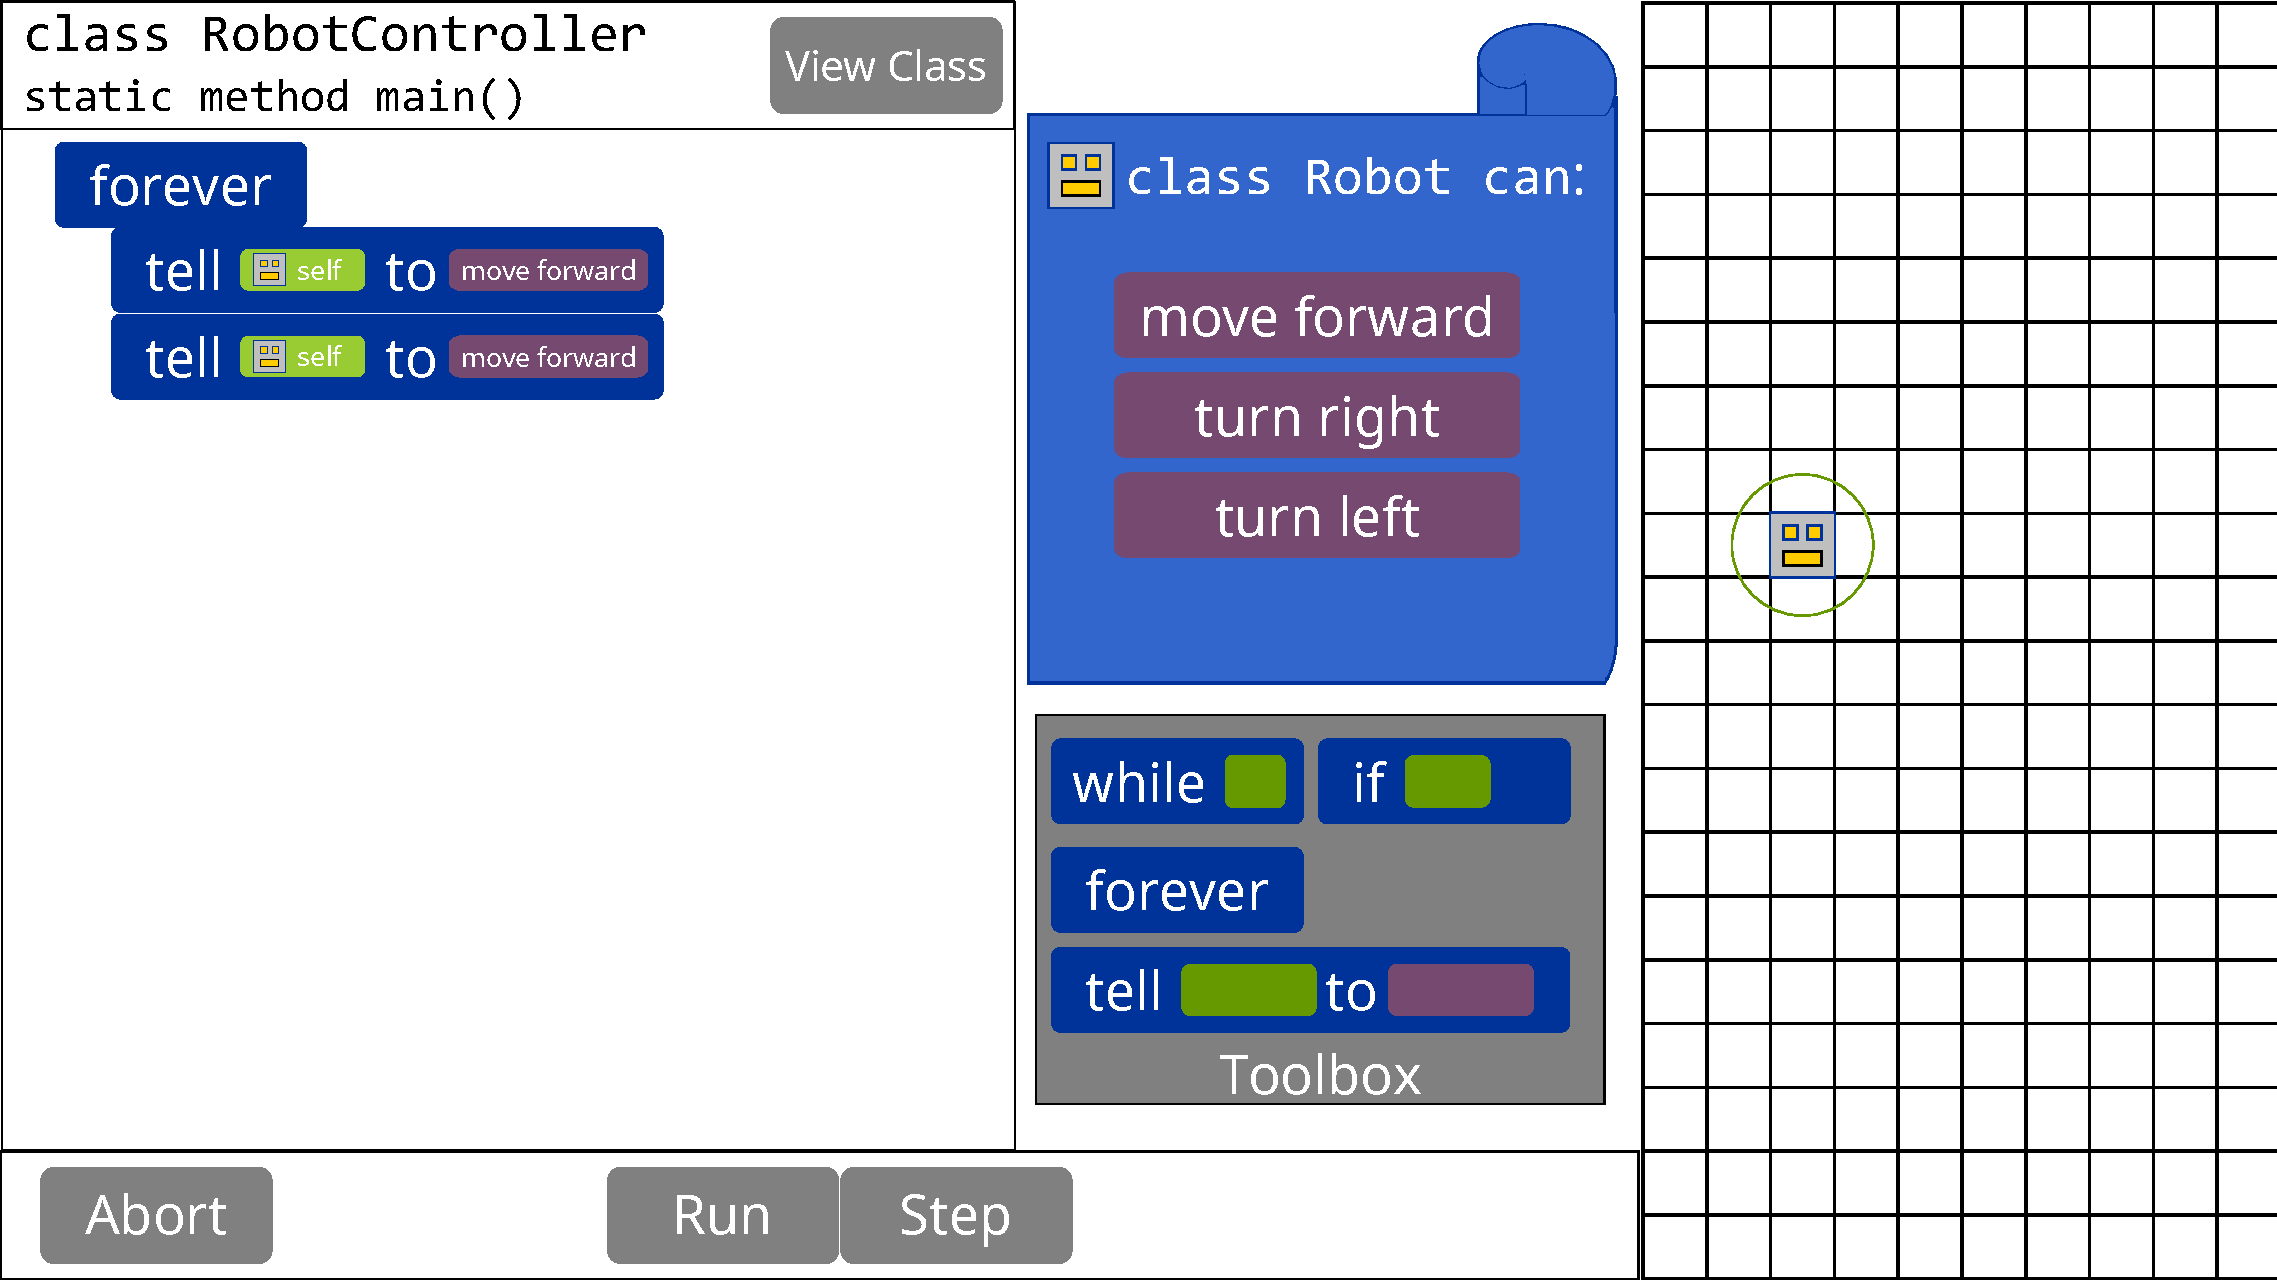
\includegraphics[width=\textwidth]{mockup.pdf}
  \caption{The main game interface.}
\end{figure}
The user interface has three main components: the world map, the
visual programmer and the interactive debugger. Normally, the student
will see only the programming and map interface, with objectives
overlaid on the map interface. Once the student runs their code, the
debugger will appear, tracing the execution of the Java code in tandem
with the world map and code blocks.

\section{Evaluation}

We intend to test the system with a group of students in a class such
as CS 2110, Advanced Placement Computer Science, or similar class
involving Java and object-oriented principles. Students could be given
a pre- and post- test asking about various concepts from this paradigm.

\end{document}
